\section{Speed Controller - PID}

The motor and the hall-sensor together show PT1 behavior. An example for the curve is given in \ref{pt1}.

\begin{figure}[ht] 
	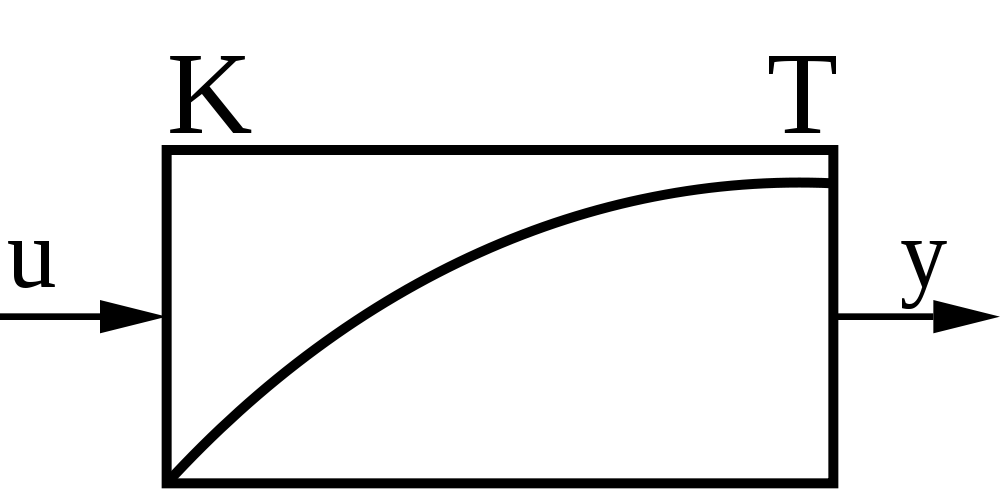
\includegraphics[width=0.5\textwidth]{figures/pt1.png}
	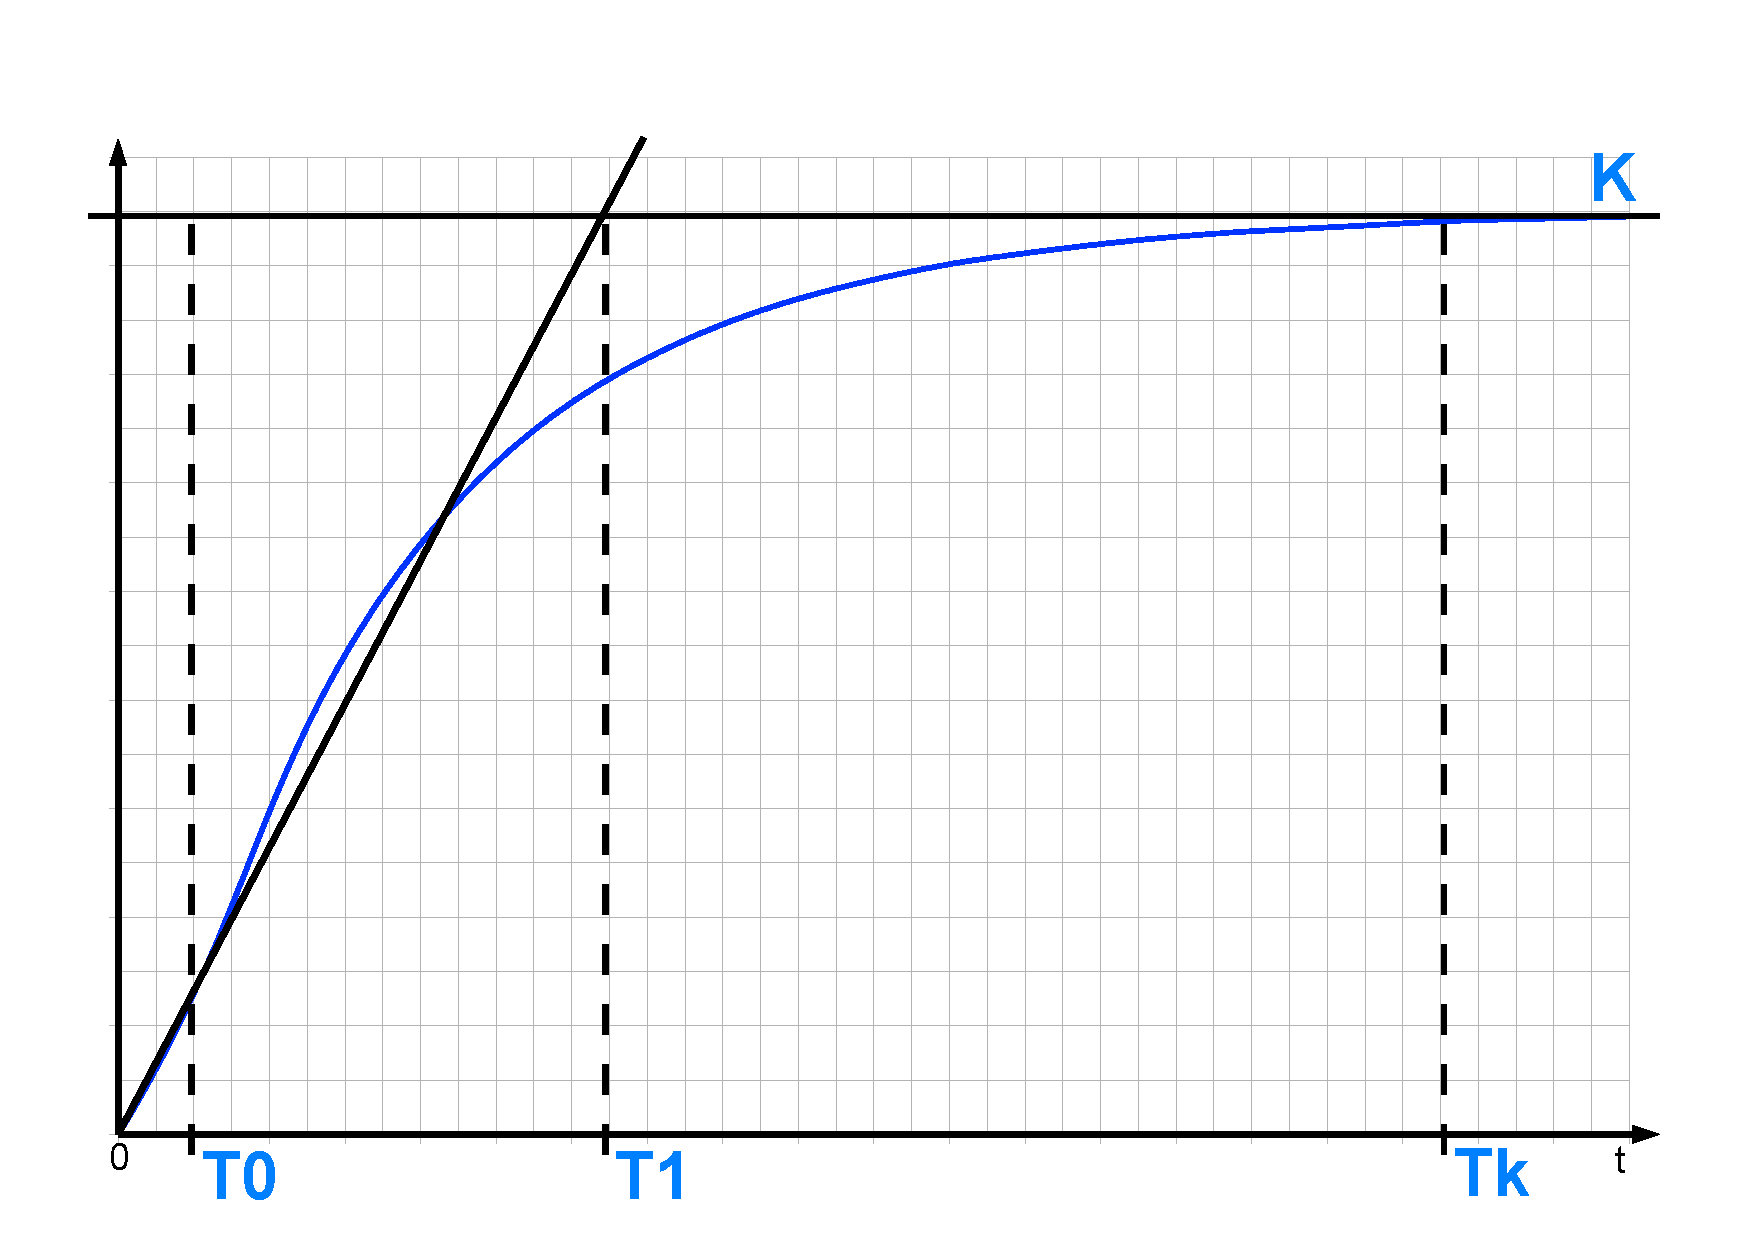
\includegraphics[width=0.5\textwidth]{figures/pt1_exact.pdf}
	\caption{Left: PT1 behavior in time domain. Right: Example for a measurement of motor + hall-sensor.} \label{pt1}
\end{figure}

To control a PT1 system you only need a PI controller. A D-value is not necessary or will have no impact on the control value.\\
The control-circle will be like \ref{circle}.

 \begin{figure}[ht] 
	\center{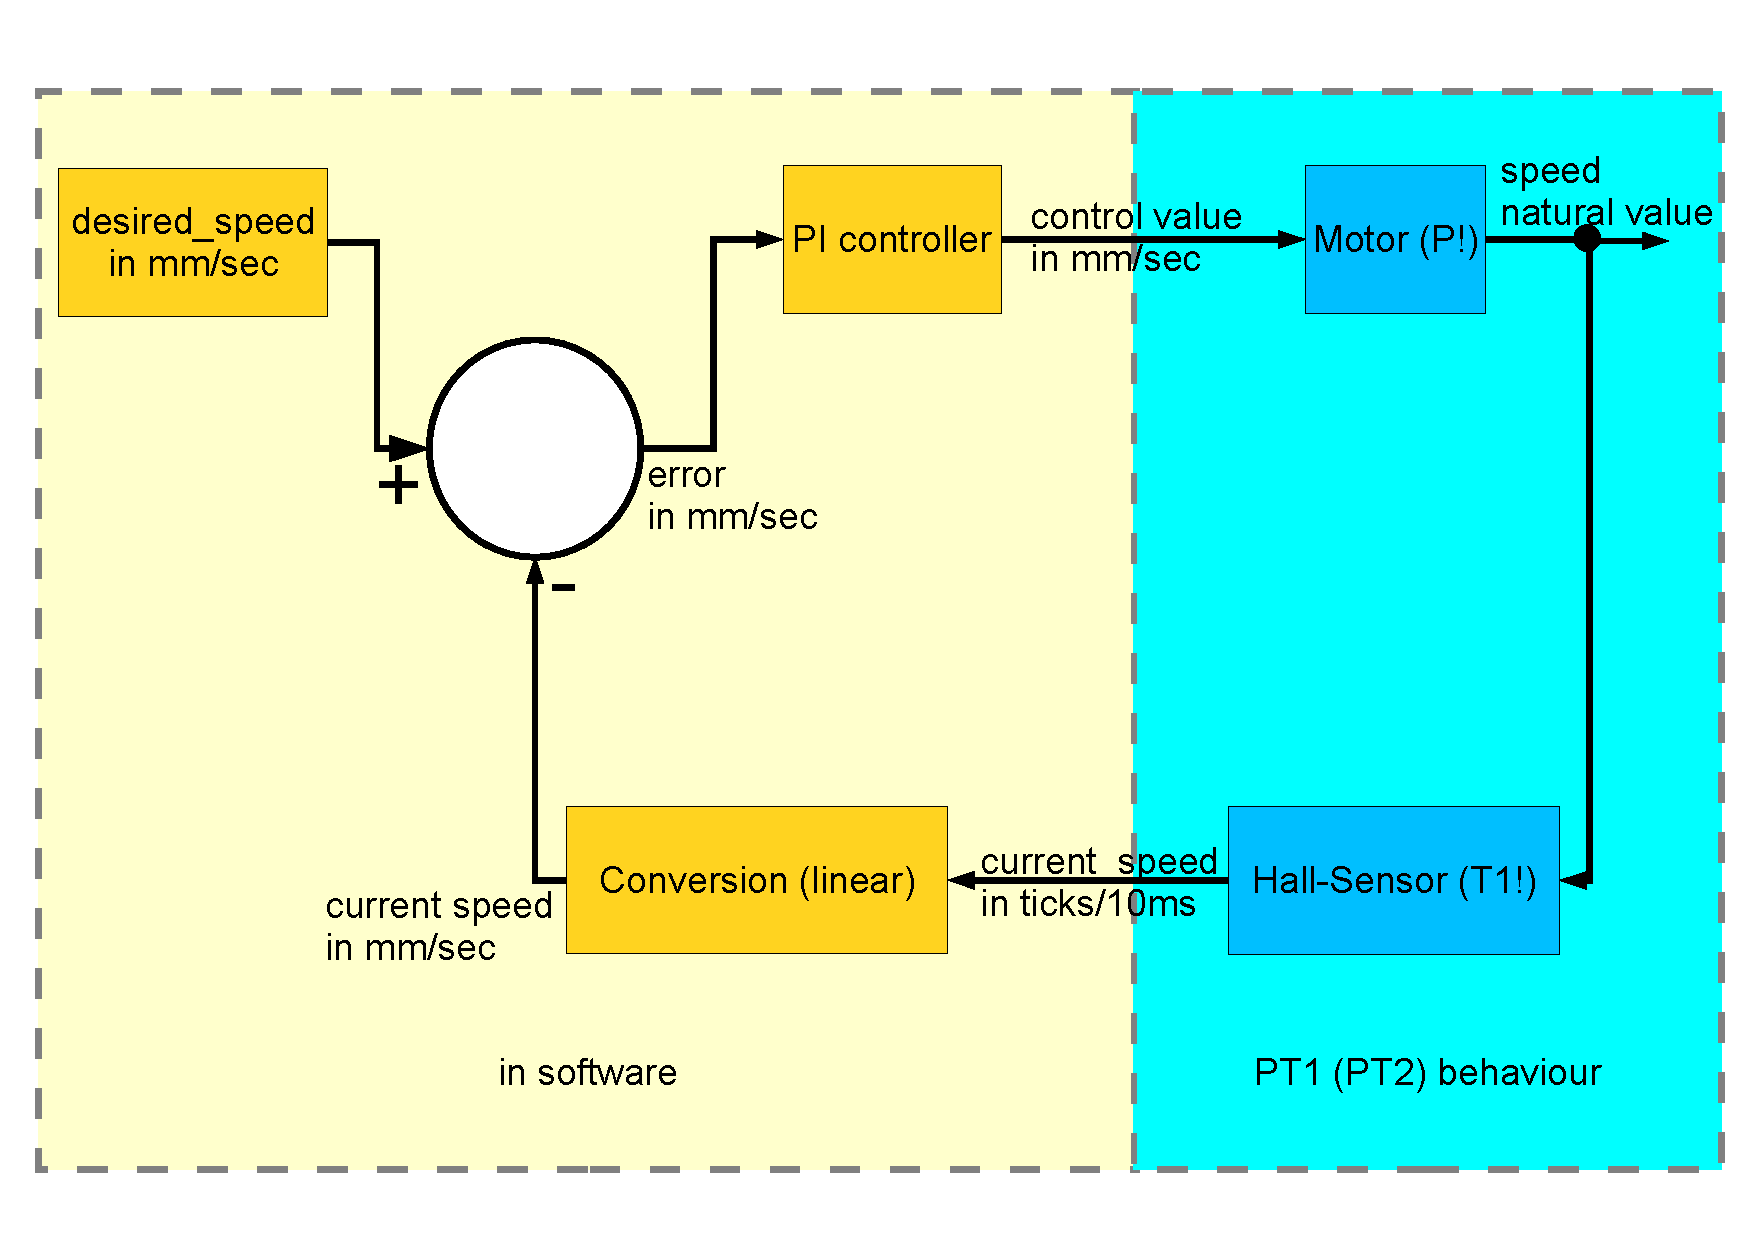
\includegraphics[width=0.6\textwidth]{figures/picontroller.pdf}}
	\caption{Control-circle with PI controller.} \label{circle}
\end{figure}


The exact transfer-functions for the motor and the hall-sensor are unknown. We assume that both have PT1 behavior. The motor dominates with his P and the sensor dominates with his T.
Together they have a dominating PT1 behavior but in the strict sense total a PT2 behavior. You can see the PT2 behavior in \ref{pt1} (right). The tangent at the origin hits the curve two times. In an PT1 system this should never happen, so we infer from that PT2 behavior.\\

Thus we can never guarantee that our PI controller produces no overshoots. The probability for this scenario may be very low and the overshoots also.\\

The controller is written in software. This causes a high discretization (error). The speed
is not controlled continuously but every 10ms. With this errors and delays the PT2 behavior
becomes more unstable. We recommend a (hardware) implementation in the FPGA. This will also not be fully continuously but will control the speed more detailed.\\

All together the system has PIT1 behavior. This means there is still a remaining delay for acceleration and slow-down!